\section{目的}
依 Lab 8（PDF 31--34 頁）求反相器 VTC、切換門檻與雜訊容限，再用有限時間擾動檢查後級恢復。

\section{Spec 對照}
\begin{longtable}{p{0.31\linewidth}p{0.29\linewidth}p{0.31\linewidth}}
\toprule
講義要求（PDF頁） & 實作 & 驗證與界線 \\\midrule
步驟 1：VTC、斜率 $-1$ 與 NM（31--33） & 01\_dc\_transfer & 中央差分與交點內插 \\
步驟 2：改變寬度比（32--33） & $W_p/W_n=0.75,3,12$ & 三組完整曲線 \\
步驟 3：各比例雜訊比較（33） & 02\_noise\_cascade & 低態正擾動、高態負擾動 \\
問題：再接 CMOS 後級（34） & 每種比例皆加第二級 & 同時保存兩級波形 \\
\bottomrule
\end{longtable}


\section{電路與設計推導}
固定 $W_n=0.6\,\mu$m、$L=0.25\,\mu$m，以 $W_p=0.45,1.8,7.2\,\mu$m 實現講義三種比例。切換門檻定義為 $V_o=V_{DD}/2$，不是單顆 MOS 的 threshold。$V_{IL},V_{IH}$ 為 $dV_o/dV_i=-1$ 的兩個交點；採邊界輸出 $V_{OH}=V_o(V_{IL})$、$V_{OL}=V_o(V_{IH})$ 計算 $NM_L=V_{IL}-V_{OL}$、$NM_H=V_{OH}-V_{IH}$。CSV 另外保存講義採理想電源軌近似的 NM，以免混用定義。修正原始只有部分斜率交點、不同尺寸分散的測試，補上完整兩種 NM 與三級比例比較。

\section{模擬設定}
本次為使用另行提供模型的教學改寫，電源為 1.0 V、溫度為 $25\,^{\circ}\mathrm C$。保留講義指定的拓樸、負載及比較尺寸；原講義的 2.5 V 製程結果不是本次模型的驗收數值。1 V 僅是模擬條件，不能視為模型的安全額定。所有 MOS 的 Bulk 明確接至相應電源軌。

HSPICE S-2021.09 使用 RUNLVL=6；保存波形、列印資料及原生量測。圖表由本次數據重繪；CSV 保存於各 Lab 的 results。完成模擬表示求解成功，並不代表製程可靠度已驗證。加密模型仍有被抑制的警告；既有診斷未取得可判讀的進一步內容，因此不宣稱警告無害或全部模型限制已滿足。

DC 為 0--1 V、0.5 mV 步距。暫態 18 ns、列印 2 ps；低態擾動 0.2/0.4/0.48/0.6 V，高態短暫降至 0.8/0.6/0.52/0.4 V，邊緣 0.1 ns、平台 0.9 ns。這是原圖雜訊概念的正規化測試，未將原 1.2/1.3 V 值冒用於 1 V。

\section{結果與規格檢查}
兩份 deck 均成功。下表所有電壓與容限單位 V，採邊界輸出定義。
\begin{center}\small
\begin{tabular}{llllll}
\toprule
$W_p/W_n$ & $V_M$ & $V_{IL}$ & $V_{IH}$ & $NM_L$ & $NM_H$ \\
\midrule
0.75 & 0.4214 & 0.3617 & 0.4496 & 0.3237 & 0.5100 \\
3 & 0.4825 & 0.4291 & 0.5189 & 0.3855 & 0.4376 \\
12 & 0.5459 & 0.5031 & 0.5925 & 0.4600 & 0.3616 \\
\bottomrule
\end{tabular}
\end{center}

\begin{figure}[htbp]
\centering
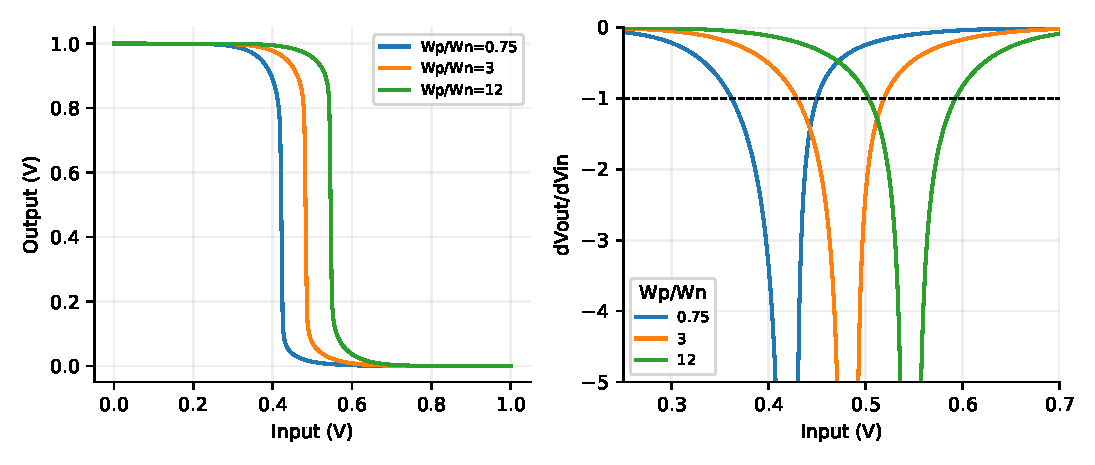
\includegraphics[width=\linewidth]{figures/inverter_transfer.pdf}
\caption{VTC 與斜率 $-1$ 的交點；由本次 HSPICE 數據重繪。}
\end{figure}

\begin{figure}[htbp]
\centering
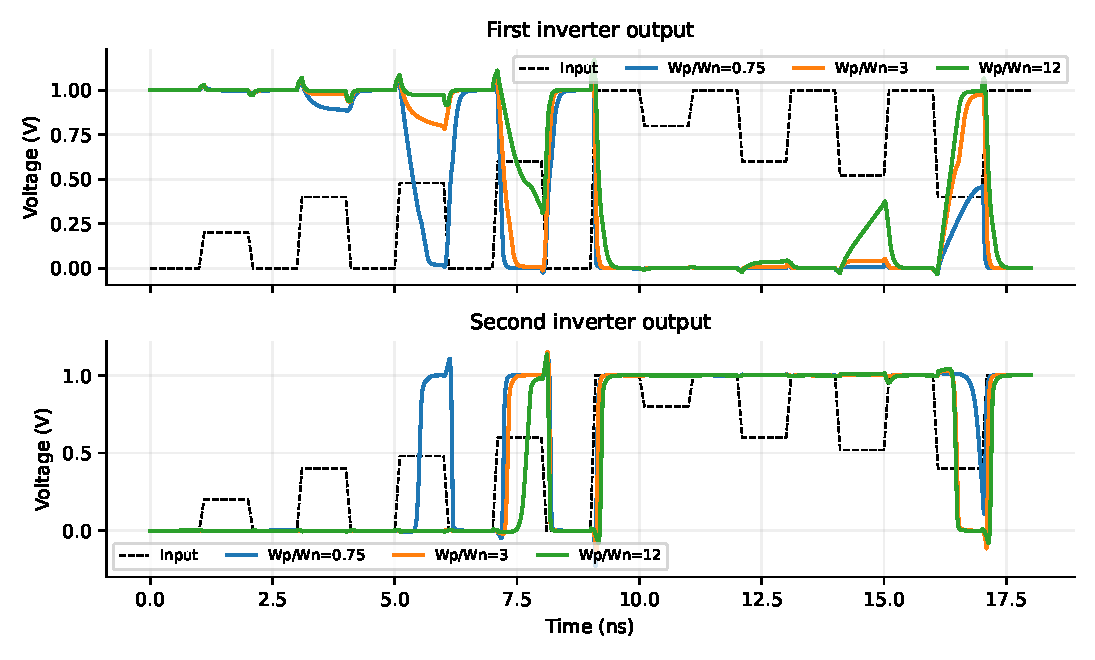
\includegraphics[width=\linewidth]{figures/noise_regeneration.pdf}
\caption{各比例的第一級及第二級雜訊響應；由本次 HSPICE 數據重繪。}
\end{figure}


\section{討論}
增加 PMOS 寬度使門檻右移，$NM_L$ 增加、$NM_H$ 減少；比例 3 在本次模型仍非完全對稱。第二級可使未跨越切換區的擾動恢復為較完整電源軌，但若第一級已因擾動改變邏輯，後級可能將錯誤放大成完整脈波。有限脈寬的濾除依賴時間與負載，不能把暫態「未翻轉」直接等同 DC noise margin。

\section{結論}
三個步驟及串接問題皆有完整模擬與量測。電壓正規化與 NM 定義差異均已揭露，未宣稱重現原製程的容限數字。
